\documentclass{article}
\usepackage{amsmath}  % needed for \tfrac, \bmatrix, etc.
\usepackage{amsfonts} % needed for bold Greek, Fraktur, and blackboard bold
\usepackage{graphicx} % needed for figures
\usepackage{gensymb}  % needed for general symbols
\usepackage{url}      % needed for citing websites
\usepackage{natbib}   % needed for bibliography 
\usepackage{flexisym} % needed for other mathematical symbols
\usepackage{siunitx}  % needed for other mathematical symbols
\usepackage{commath}  % needed for mathematical symbols
\usepackage[utf8]{inputenc}

%% Resources: 1. Fluroscent light spectrum literature https://www.researchgate.net/figure/a-Spectrum-of-light-emission-from-fluorescent-room-lights-b-Spectrum-of-sunlight_fig2_225633277
%% 2. Florescent light spectrum file:///Users/CocoLelio/Downloads/sensors-10-03961.pdf
%% 3. Two pictures side by side https://tex.stackexchange.com/questions/37581/latex-figures-side-by-side


\title{Spectroscopy Laboratory Report}
\author{Ke Li, Jerome Jahn }
\date{February 2019}

\begin{document}
\maketitle

\tableofcontents
\clearpage

\section{Introduction}
This set of experiments was aimed at exploring various aspects of spectroscopy. A spectrometer outputting into the Ocean Optics SpectraSuite software was used to capture emission, absorbance and transmission spectra. The investigations included determining the effect of the integration time of a CCD on the captured spectra, comparing the emission spectra of various light sources, determining the spectral characteristics of colored glass filters and determining the effect of the concentration of color additives in solution on the absorbance of that solution for the given color.

\section{Theory}
\subsection{Spectroscopy}
Spectroscopy is the scientific study of spectra of light. A spectrum is a graphical representation of the spectral components of light. In considering the shape of a captured spectrum, the pathway of the light to the detector needs to be considered. Naturally, the pathway of light begins with its emission from a particular source. After emission, light-matter interaction can change the spectrum. Lastly, the interaction of the light with the detector gives the spectrum its final shape.  
\subsection{Emission of Electromagnetic Radiation}
Emission sources vary in their emitted spectra. Fundamentally, all emissions of light from a source are linked to a change in the energy state of one or more of the particles of the emitting material. Each energy level change corresponds to the creation of a photon. Disregarding frequency shifts due to the relativistic Doppler effect, the energy within the photon is directly proportional to that photon's frequency. Equation (1) shows the direct relationship mentioned above

\begin{equation}
    E = hf.
\end{equation}

$E$ is the energy in Joules, $f$ is the frequency of light in $m^-1$, and $h$ is Planck's constant with a value of $6.626 070(15) \times 10^-34 J/s$ \cite{units}. 

\subsection{The Two-Level System}
The energy that goes into the creation of a photon is in some cases due to an electronic energy level transition. Disregarding the relativistic Doppler effect once again, the energy carried by the photon is exactly equal to the energy difference between the initial electron energy and the final electron energy. This is represented by equation [2] below

\begin{equation}
    hv = \Delta E = \abs{E_i - E_k}.
\end{equation}

When considering a simple two-level system, where the electron has the option of being on one of two nondegenerate energy levels, there are two overall possibilities -- absorption of a photon by the electron to go from the lower energy level to the higher one and emission of a photon when the electron drops from the higher one to the lower one. The possibilities are shown in figure~\ref{fig:two_level}.



\begin{figure} [h!]
    \centering
    \includegraphics[width=3in]{Two_Level_System.PNG}
    \caption{Electronic Energy Transitions in a Two Level System}
    \label{fig:two_level}
\end{figure}

The two energy levels are separated by the energy difference $\Delta E = E_i - E_j$. Possible electronic energy transitions are spontaneous emission  $A_{ik}$, where the electron drops from the higher energy level $E_i$ to the lower energy level $E_k$ and emits a photon, absorption $B_{ki}$, where the electron absorbs a photon with energy equal to the energy difference $\Delta E$, or stimulated emission $B_{ik}$, where a passing photon causes an energy level change from $E_i$ down to $E_k$ and the emitted photon adds constructively with the passing photon.

The emission spectrum of a two level system is a single wavelength. A material has multiple energy levels that electrons can jump between. When the material has excited electrons, which were excited by The emission of light due to these jumps forms a discrete emission spectrum. Furthermore, when a continuous spectrum is incident on a material with such quantized energy levels, certain photons corresponding to the energy difference between the levels will be absorbed. The spectrum, after passing through this material, will have absorption lines, or "holes," corresponding to these absorbed photons.

Actual observed spectra are subject to line broadening. This line broadening takes the shape of making a peak a Lorentzian, Gaussian, or a convolution of both called a Voigt profile. The shapes are shown in figure~\ref{fig:gaussian and lorentzian}.

\begin{figure} [h!]
    \centering
    \includegraphics[width=2in]{Gaussian_Lorentzian.PNG}
    \caption{A Gaussian, Lorentzian and Voigt Lineshape}
    \label{fig:gaussian and lorentzian}
\end{figure}

Lorentzian lineshapes are much narrower than Gaussian lineshapes of the same height. Lorentzian lineshapes are due to natural broadening stemming from the Heisenberg uncertainty principle. This natural broadening is ever present, no matter the emission source. Lorentzian lineshapes can also be influenced by collisional broadening. When gas atoms collide, the kinetic energy from one atom can change the energy of the electrons of the other. This results in a broader lineshape. Gaussian lineshapes are due to the thermal motions of electrons resulting in a frequency shift due to the relativistic Doppler effect. Voigt profiles are due to the presence of the conditions necessary for both lorentzian and gaussian lineshapes.

A second kind of important emission spectrum is the continuous spectrum stemming from black-body radiation. The distribution of the emitted wavelengths follows Planck's law, written in Equation (3)

\begin{equation}
    W_v (v) dv = \frac{8\pi h v^3}{c^3} \frac{dv}{ e^{\frac{hv}{kT} -1 }},
\end{equation}

where $W_v(v)$ is the spectral density. As can be seen from the equation, the emission spectrum is continuous and depends on the temperature of the emission body.
General black-body radiation spectrum is shown from the figure below.\cite{black_body} In practice, solid, liquid and high pressured vapor will generate continuous spectrum due to thermal radiation. Based on this theory, we used halogen lamp which can generate continuous spectrum for spectrum measurement.  

\begin{figure}[h!]
    \centering
    \includegraphics[width = 3.0 in]{blackbody.jpg}
    \caption{Black-body Radiation Spectrum}
    \label{fig:black_body}
\end{figure}

\subsection{Beer-Lambert Law and Absorbance}

Beer- Lambert Law connects the attenuation of a light source when light travels through an absorbing material. It can relates the transmission of the intensity of the light to the material property that the light travels through and the depth of the material the the light penetrates through.

There are three major forms of light-matter interactions: transmission, absorption, and reflection. The general light-matter interaction can be expressed by the complex refractive index:

\begin{equation}
    N = n + i\kappa
\end{equation}

where n is the refractive index in the spectral region where the material appears to be transparent to the light source, and $\kappa$ is the extinction coefficients that relates to the energy loss, also known as the absorption of the light source in the material. From this complex refractive index, we could find the absorption coefficient of the material, which is defined as:

\begin{equation}
    \alpha = \frac{4\pi \kappa}{\lambda_0}
\end{equation}
where $\lambda_0$ is the wavelength is vacuum.

In a solution, the absorption coefficient is defined as:

\begin{equation}
    \alpha = \epsilon_l c
\end{equation}

where $\epsilon_l$ is the extinction coefficient of the solution, and c is the concentration of the solution.

The Beer-Lambret Law states that: 

\begin{equation}
    \frac{\Delta I }{I_0} = - \alpha \Delta b
\end{equation}

where $I_0$ is the initial light intensity before going through the material, $\Delta I $ the change of intensity when the light pass through $\Delta b$ depth of the material. 

The final Beer-Lambret Law after integration on both side yields:

\begin{equation}
    I(b) = e^{-\alpha b}
\end{equation}

Based on the definition of light transmission through a material, which is the ratio of the intensity of light actually passing through the material, and  the initial intensity of the light, we can derive the definition of an important property of spectroscopy: the absorbance.

\begin{equation}
    A = log_{10} (\frac{1}{T}) =  \epsilon c b
\end{equation}

where $T$ is the transmission coefficient of the material, c the concentration of the solution, and $\epsilon$ the wavelength dependent absorption coefficient of the solution. From the equation above, we can determine the concentration of a solution to the absorbance measured from a spectrum.

\begin{equation}
    c = \frac{A}{\epsilon b}
\end{equation}

The transmission of the material $T$ is defined as the ratio of the transmitted intensity of light to the initial intensity of the light.

Since absorbance of a solution and the concentration of the solution has linear connection, we can estimate coefficient $\epsilon$ with multiple measurements of $c$ and $A$ of the solution. 


\subsection{Spectrometer}

\subsubsection{General Set up}
Optical spectrometer is a device designed to record the intensity distribution of a light source according to their wavelengths. As Figure ~\ref{fig:spectrometer_setup} shows, a spectrometer is composed of a collimating mirror that collimates the incoming light from light source to the grating component. The grating component decompose the collimated light source into component of various wavelengths. The dispersed light travels to a focusing mirror, after which the focused light is then detected at the exit slit by a CCD camera or other light detecting sensor.  

\begin{figure}[h!]
    \centering
    \includegraphics[width = 3.5 in]{spectrometer.png}
    \caption{Spectrometer setup}
    \label{fig:spectrometer_setup}
\end{figure}


From the fundamentals of geometry, we may find the relation between spacial separation $\Delta x$ and the wavelength distance $\Delta \lambda$:

\begin{equation}
    \Delta x = x(\lambda + \Delta \lambda) - x(\lambda) = f_{2}\frac{d_{y_{g}}}{d\lambda} \Delta \lambda
\end{equation}

where $f_2$ is the focal length of the collimated and focusing lenses of the system, and $\frac{dy}{d \lambda}$ is the dispersion of of the grating, where $g$ is the grating index. Even though there are different mechanisms to decompose light components, a grating sepctrometer was used in this experiment, due to higher resolution of wavelength that the spectrometer can detects.

The spectral resolution of a grating spectrometer is given as:

\begin{equation}
    R = m \times K
\end{equation}

where m is the interference order, and K is the number of illuminated grating grooves.

\subsubsection{Emission, Absorbance, and Transmission Spectrum}

An optical spectrometer can be used to record different spectrum that result from different kinds of light matter interaction.

%Add citation : https://www.comsol.com/blogs/calculating-the-emission-spectra-from-common-light-sources/%
Figure ~\ref{fig:Fluorescent_Bulb} below is a typical emission spectrum of a fluorescent light bulb. From an emission spectrum, we can analyze the wavelength components of the light source. In this example, we can conclude from the emission spectrum that the energy emission of a fluorescent light bulb is quantized, resulting in several peaks at certain wavelengths.     

\begin{figure}
    \centering
    \includegraphics[width = 3 in]{Emission-spectrum-of-fluorescent-bulb.png}
    \caption{Emission Spectrum of Fluorescent Bulb}
    \label{fig:Fluorescent_Bulb}
\end{figure}

%https://www.researchgate.net/figure/Typical-absorption-spectrum-of-Silver-Island-Films-SiFs_fig1_8021106

Figure ~\ref{fig:Typical Absorption Spectrum} below shows a typical absorption spectrum measured by spectroscopy.  Unlike an emission of a light source, the absorption spectrum, especially in a solution, has the feature of broad band instead of spectrum with distinguishable peaks. This is due to the fact that the absorbing molecule in a solution is surrounded by solvent molecules, which constantly dissolve and rejoin. This affect the energy level of the molecules differently for different absorbing components in the solution, resulting in a broad band spectrum.



\begin{figure}[h!]
    \centering
    \includegraphics[width = 3 in]{Typical-absorption-spectrum-of-Silver-Island-Films-SiFs.png}
    \caption{Typical Absorption Spectrum}
    \label{fig:Typical Absorption Spectrum}
\end{figure}


Figure ~\ref{fig:Longpass} below shows a typical transmission spectrum of a filtered glass. Based on the range of wavelength the different filter transmits through, transmission spectrum can be categorized as long pass filter and band pass filter. Figure ~\ref{fig:Longpass} is an example of long pass filter.

\begin{figure}[h!]
    \centering
    \includegraphics[width = 3 in]{Filter_2_Transmission_Spectrum.png}
    \caption{A Long Pass Transmission Spectrum}
    \label{fig:Longpass}
\end{figure}
\subsection{Colored Light Emitting Diodes (LEDs)}

Light Emitting Diodes (LEDs) are important semiconductor devices. The LED consists of a p-n junction. Upon application of a current across the junction, electrons from the n-doped semiconductor travel to the p-doped semiconductor and fall into the valence band. This energy transition causes an emission of light. The peaks in the spectrum of the LED correspond to the energy difference between the conduction band and the valence band. This energy difference can be tuned for a particular wavelength by tuning the semiconductor's material properties.

The peak in the emission spectrum of the LED is much narrower due to this tuning of the bandgap. Typical emission spectra of colored LED's are shown in figure~\ref{fig:Led spectra} \cite{spectra}.

\begin{figure}[h!]
    \centering
    \includegraphics[width = 3 in]{LED_spectra.PNG}
    \caption{LED Spectra}
    \label{fig:Led spectra}
\end{figure}
\subsection{White LED and Fluorescent Room Lights}
White LEDs and fluorescent mercury vapour lamps are two options for room lighting in a laboratory. The spectra of these two are shown in figure~\ref{fig:room lighting spectra} \cite{spectra}.

\begin{figure}[h!]
    \centering
    \includegraphics[width = 3 in]{lighting_spectra.PNG}
    \caption{Typical Room Lighting Spectra}
    \label{fig:room lighting spectra}
\end{figure}

\subsection{Lasers}
Lasers have very narrow linewidths. They take on a Gaussian form. Two important lasers are the green frequency-doubled ND:YAG laser and the red diode laser. Typical emission spectra of these two are shown in figure and figure .

\begin{figure}[h!]
    \centering
    \includegraphics[width = 3 in]{LED_spectra.PNG}
    \caption{LED Spectra}
    \label{fig:Led spectra}
\end{figure}
\section{Experimental Procedures}
\subsection{General Setup}
The general setup consisted of an emission source shining light into optical fibers that led into a Red Tide USB650 grating spectrometer. The grating spectrometer had a CCD camera that converted incident photons on its pixels into counts that were communicated with a USB cable to a Windows computer running the Ocean Optics SpectraSuite software. Figure~\ref{fig:real setup} below shows a picture of the general setup. 

\begin{figure} [h!]
    \centering
    \includegraphics[width=2in]{RealSetup.jpg}
    \caption{Experimental Setup}
    \label{fig:real setup}
\end{figure}

In the picture a halogen lamp is being used as a light source, and a stage that can be used to filter the emission source's light has been inserted between the lamp and the spectrometer. The inside of the spectrometer is shown in Figure~\ref{fig:grating spectrometer} below. 

\begin{figure} [h!]
    \centering
    \includegraphics[width=2in]{Grating_Spectrometer.PNG}
    \caption{The Interior of the Grating Spectrometer. Image taken from Lab Handout.}
    \label{fig:grating spectrometer}
\end{figure}

The optical cable  shines light onto a mirror which reflects it onto a grating. The second diffraction order lands on a second mirror and is reflected onto a detector, in this case a CCD camera. The grating spatially separates the wavelengths within the signal and leads them onto different pixels in the CCD. This is shown in Figure~\ref{fig:ocean optics spectrometer} below.

\begin{figure} [h!]
    \centering
    \includegraphics[width=2in]{OceanOpticsSpectrometer.PNG}
    \caption{Ocean Optics Spectrometer}
    \label{fig:ocean optics spectrometer}
\end{figure}

In the experiments that follow, a color filter or color additive solution is placed in the filtering stage and analyzed in the SpectraSuite software. A schematic of the general setup is shown in Figure~\ref{fig:optical setup schematic} below.

\begin{figure} [h!]
    \centering
    \includegraphics[width=2in]{Optical_Setup_General.png}
    \caption{General Setup for all Experiments.}
    \label{fig:optical setup schematic}
\end{figure}

The straight lines in the figure above represent light transmission through optical fibers, whereas the curved line represents the output of the CCD being communicated to a computer with an electronic cable. Light is generated in the emission source, can be filtered by the color filter or color additive solution, and is analyzed by the spectrometer. The SpectraSuite software is able to tune the integration time of the CCD and can compute absorption and transmission spectra from the measured spectrum on the CCD, which is given in counts per wavelength. 

\subsection{CCD Integration Time Investigation}
The first part of the experiment involved determining the effect of changing the integration time of the CCD in the SpectraSuite software. The spectrum of a halogen lamp was recorded with an integration time of 100 milliseconds. The integration time was incrementally decreased until it was at 20 milliseconds, with the effect being determined. At 20 milliseconds the halogen lamp spectrum was once again recorded. 


\subsection{Absorption and Transmission of Colored Glass Filters}
A Thorlabs FGK01S set of 10 2" by 2" square colored filters was investigated. First, the shutter on the halogen lamp was shut and the dark spectrum was recorded. The spectrum of the halogen lamp was recorded with the dark spectrum subtracted. Filter 1, a filter transparent to all wavelengths of light able to be analyzed by the Red Tide USB650 spectrometer, was put into the filter slot as a reference filter. As it was noticed that any tilt to the filter would alter the shape of the spectrum, the group chose to stand the filter upright and flush against the lower side of the filter stage, as shown in Figure~\ref{fig:colored filter} below.

\begin{figure} [h!]
    \centering
    \includegraphics[width=2in]{Filter1.jpg}
    \caption{Method of Placing Color Filters in Holder}
    \label{fig:colored filter}
\end{figure}

All filters were placed like this into the stage in order to avoid this source of error. The reference spectrum was saved into the program. The group recorded the spectrum, absorption spectrum, and transmission spectrum of filters labeled two, three, four and five. From the transmission spectra on SpectraSuite, these were classified as either bandpass or longpass optical filters. Using the spec sheet of the optical filter kit, the filters were matched according to their transmission spectra with the filter's product numbers as listed by ThorLabs. Two longpass filters, Filters 3 and 4, were used at the same time in order to determine the effect on the cutoff wavelength. Lastly, using trial and error, a bandpass filter passing light roughly in the 500-700 nanometers was created by using two of the filters in the kit. 


\subsection{Absorption in Color Additive Solutions}
The second part of the experiment involved placing color additive solutions filled into a cuvette in the filtering stage and measuring the resulting absorption spectra. A halogen lamp was used as a light source. A reference spectrum was found by placing a cuvette filled with 1 mL of water into the filtering stage and saving the reference spectrum into the program. Then .2 mL of blue food coloring was added to the cuvette. When the solution was homogeneous, the cuvette was placed into the filtering stage and the absorption spectrum was recorded. This was repeated until the total volume of the solution in the cuvette was 2 mL. A cuvette with an unknown amount of blue food coloring mixed with water was then placed into the filtering stage. The absorption spectrum was recorded. 

The effect of mixing two color additives into the same solution was investigated next. The colors used were red and purple. Two cuvettes were prepared, both containing a solution that had 1 mL of water and roughly .5 mL of the respective color additive. The group was only interested in the location of the peaks of the absorption spectrum. Next, roughly .5 mL of purple dye was added to the cuvette containing the red solution. The absorption spectrum of this new solution was recorded.

\subsection{Emission Spectra of Light Sources}
%% LED Spectrum https://www.comsol.com/blogs/calculating-the-emission-spectra-from-common-light-sources/
The third part of the experiment consisted of measuring the emission spectra of various sources in order to qualitatively compare them. The filtering stage was omitted for these measurements, and the light of the sources was coupled into the fiber by aiming the fiber at the various sources. The spectra which the group recorded were of a halogen lamp, room light, white LED, yellow LED, red LED, blue LED, iPhone 6+ LED flashlight, Samsung S8 LED flashlight, blue LED on the Cooler Master desktop,  red laser, green laser, and the LCD computer monitor showing the color white.. The spectra were then analyzed for their relative peaks and the reasons for these peaks.



\section{Results}
\subsection{CCD Integration Time Investigation Results}
Longer integration times lead to higher photon counts in a linear manner. Furthermore, pixel saturation for a given wavelength manifesting itself at around 4000 counts was observed for integration times that were too high given the source brightness. Besides there being a maximum number of counts able to be registered by the CCD, there was a roughly direct proportionality observed between the integration time and the counts per wavelength. The characteristic peaks of the spectrum did not change and their relative intensities were not impacted by the integration times, with the exception of the wavelengths that had reach the maximum photon counts. The signal-to-noise ratio was not observed to necessarily increase with higher integration times.

\subsection{Absorption and Transmission of Colored Glass Filters Results}

\subsubsection{Software Setup}

The group obtained the dark spectrum shown in Figure~\ref{fig:dark spectrum} below.
\begin{figure} [h!]
    \centering
    \includegraphics[width=2in]{Dark_Spectrum.png}
    \caption{Dark Spectrum of CCD}
    \label{fig:dark spectrum}
\end{figure}

The halogen lamp spectrum taken after the dark spectrum was subtracted is shown in Figure~\ref{fig:halogen lamp spectrum} below.

\begin{figure} [h!]
    \centering
    \includegraphics[width=2in]{Halogen_Emission_Spectrum.png}
    \caption{Halogen Emission Spectrum}
    \label{fig:halogen lamp spectrum}
\end{figure}

The reference filter spectrum is shown in Figure~\ref{fig:filter 1 reference spectrum} below.

\begin{figure} [h!]
    \centering
    \includegraphics[width=2in]{Reference_Halogen_Lamp_S_Spectrum.png}
    \caption{Reference Spectrum}
    \label{fig:filter 1 reference spectrum}
\end{figure}

\subsubsection{Filter 2 Identification}
The spectrum of Filter 2 is shown in Figure~\ref{fig:filter 2 S spectrum} below.

\begin{figure} [h!]
    \centering
    \includegraphics[width=2in]{Filter_2_S_Spectrum.png}
    \caption{Halogen Lamp with Filter 2 Spectrum}
    \label{fig:filter 2 S spectrum}
\end{figure}

The absorbance spectrum of Filter 2 is shown in Figure~\ref{fig:filter 2 A spectrum} below.

\begin{figure} [h!]
    \centering
    \includegraphics[width=2in]{Filter_2_Absorbance_Spectrum.png}
    \caption{Filter 2 Absorbance Spectrum}
    \label{fig:filter 2 A spectrum}
\end{figure}

The transmission spectrum of Filter 2 is shown in Figure~\ref{fig:filter 2 T spectrum} below.

\begin{figure} [h!]
    \centering
    \includegraphics[width=2in]{Filter_2_Transmission_Spectrum.png}
    \caption{Filter 2 Transmission Spectrum}
    \label{fig:filter 2 T spectrum}
\end{figure}

This transmission spectrum is characteristic of a longpass wavelength filter. When compared to the spec sheet from ThorLabs, this resembled the transmission spectrum of FGL495S.

\subsubsection{Filter 3 Identification}
The spectrum of Filter 3 is shown in Figure~\ref{fig:filter 3 S spectrum} below.

\begin{figure} [h!]
    \centering
    \includegraphics[width=2in]{Filter_3_S_Spectrum.png}
    \caption{Filter 3 Spectrum}
    \label{fig:filter 3 S spectrum}
\end{figure}

The absorbance spectrum of Filter 3 is shown in Figure~\ref{fig:filter 3 A spectrum} below.

\begin{figure} [h!]
    \centering
    \includegraphics[width=2in]{Filter_3_Absorbance_Spectrum.png}
    \caption{Filter 3 Absorbance Spectrum}
    \label{fig:filter 3 A spectrum}
\end{figure}

The transmission spectrum of Filter 3 is shown in Figure~\ref{fig:filter 3 T spectrum} below.

\begin{figure} [h!]
    \centering
    \includegraphics[width=2in]{Filter_3_Transmission_Spectrum.png}
    \caption{Filter 3 Transmission Spectrum}
    \label{fig:filter 3 T spectrum}
\end{figure}

This transmission spectrum is characteristic of a longpass wavelength filter. When compared to the spec sheet from ThorLabs, this resembled the transmission spectrum of FGL550S.

\subsubsection{Filter 4 Identification}

The spectrum of Filter 4 is shown in Figure~\ref{fig:filter 4 S spectrum} below.

\begin{figure} [h!]
    \centering
    \includegraphics[width=2in]{Filter_4_S_Spectrum.png}
    \caption{Filter 4 Spectrum}
    \label{fig:filter 4 S spectrum}
\end{figure}

The absorbance spectrum of Filter 4 is shown in Figure~\ref{fig:filter 4 A spectrum} below.

\begin{figure} [h!]
    \centering
    \includegraphics[width=2in]{Filter_4_Absorbance_Spectrum.png}
    \caption{Filter 4 Absorbance Spectrum}
    \label{fig:filter 4 A spectrum}
\end{figure}

The transmission spectrum of Filter 4 is shown in Figure~\ref{fig:filter 4 T spectrum} below.

\begin{figure} [h!]
    \centering
    \includegraphics[width=2in]{Filter_4_Transmission_Spectrum.png}
    \caption{Filter 4 Transmission Spectrum}
    \label{fig:filter 4 T spectrum}
\end{figure}

This transmission spectrum is characteristic of a longpass wavelength filter. When compared to the spec sheet from ThorLabs, this resembled the transmission spectrum of FGL610S.

\subsubsection{Filter 5 Identification}
The spectrum of Filter 5 is shown in Figure~\ref{fig:filter 5 S spectrum} below.

\begin{figure} [h!]
    \centering
    \includegraphics[width=2in]{Filter_5_S_Spectrum.png}
    \caption{Filter 5 Spectrum}
    \label{fig:filter 5 S spectrum}
\end{figure}

The absorbance spectrum of Filter 5 is shown in Figure~\ref{fig:filter 5 A spectrum} below.

\begin{figure} [h!]
    \centering
    \includegraphics[width=2in]{Filter_5_Absorbance_Spectrum.png}
    \caption{Filter 5 Absorbance Spectrum}
    \label{fig:filter 5 A spectrum}
\end{figure}

The transmission spectrum of Filter 5 is shown in Figure~\ref{fig:filter 5 T spectrum} below.

\begin{figure} [h!]
    \centering
    \includegraphics[width=2in]{Filter_5_Transmission_Spectrum.png}
    \caption{Filter 5 Transmission Spectrum}
    \label{fig:filter 5 T spectrum}
\end{figure}

This transmission spectrum is characteristic of a longpass wavelength filter. When compared to the spec sheet from ThorLabs, this resembled the transmission spectrum of FGL780S.

\subsubsection{Effects of Two Filters}

The group combined Filters 3 and 4 and recorded the transmission spectrum shown in Figure~\ref{fig:filter 34 T spectrum} below.

\begin{figure} [h!]
    \centering
    \includegraphics[width=2in]{Filter_34_Transmission_Spectrum.png}
    \caption{Combination of Filter 3 and Filter 4 Transmission Spectrum}
    \label{fig:filter 34 T spectrum}
\end{figure}

The new cutoff wavelength was measured to be at $590 \pm 10 $ nanometers.

In order to create a bandpass filter that passed wavelengths between 500 and 700 nanometers, the group combined Filters 2 and 7. The transmission spectrum is shown in Figure~\ref{fig:filter 27 T spectrum} below.

\begin{figure} [h!]
    \centering
    \includegraphics[width=2in]{Filter_27_Transmission_Spectrum.png}
    \caption{Filter 2 and Filter 7 Transmission Spectrum}
    \label{fig:filter 27 T spectrum}
\end{figure}

%%%
\subsection{Absorption in Color Additive Solutions Results}

The width of the plastic cuvette we used is $5 \pm 0.1 $mm, the absorption spectrum we measured for blue-dyed solution with different concentration excluding the noisy sepctral ranges is shown in the Figure ~\ref{fig:blue_dye} below. 

\begin{figure}[h!]
    \centering
    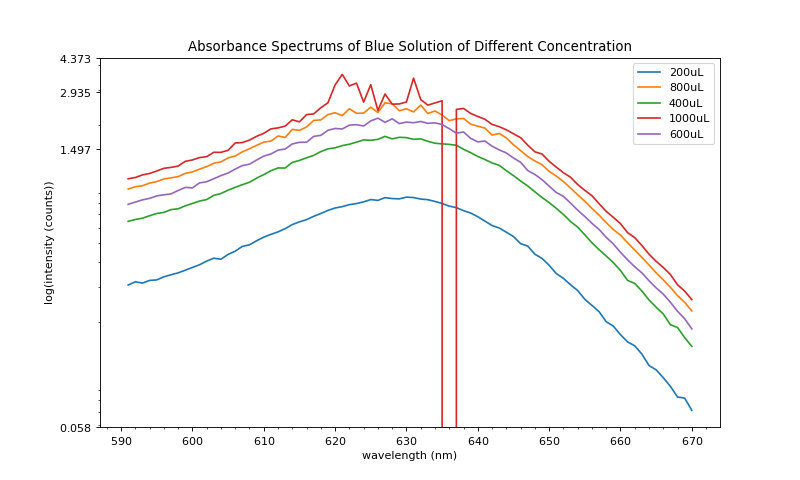
\includegraphics[width = 4.5 in ]{blue solution absorbance result.png}
    \caption{Absorption Spectrum of Blue Dyed Solution with Different Concentration }
    \label{fig:blue_dye}
\end{figure}

 We can calculate the transmission of each solution from the relation below:

\begin{equation}
    T= \frac{I_{T}- I_{d}}{I_{0} - I_{d}}    
\end{equation}

where $I_{T}$ can be calculated from subtracting the reference water spectrum and the absorption spectrum. 

With the transmission of each solution, we could find the abosrbance of the solution with the relation below:

\begin{equation}
    A = log(\frac{1}{T})
\end{equation}

For each solution, we selected the peak value of the spectrum and their corresponding wavelength to measure the absorbance of the solution. The result of wavelength , maximum intensity, reference intensity, dark intensity , transmission,and absorbance, to the corresponding solution were calculated by Python and is shown in the Table ~\ref{tab:Blue_solution} below. 



\begin{table}[h!]
    \centering
    \begin{tabular}{|c|c|c|c|c|c|}
        \hline
       Solution  & 200 micro & 400 micro & 600 micro & 800 micro & 1000 micro\\
       \hline
       Wavelength nm & 630$\pm 5$ & 627$\pm 5$ & 626$\pm 5$ & 627$\pm 5$ & 627$\pm 5$\\
       \hline
       Absorption Intensity& 0.857 & 1.743 & 2.156 & 2.579 &2.858 \\
       \hline
       Reference Intensity & 3.763 & 3.722 & 3.744 & 3.722 & 3.753\\
       \hline
       Absorbance & 0.1122 & 0.274 & 0.3724 & 0.5127 &0.6225\\
       \hline
    \end{tabular}
    \caption{Experiment Data of Blue Dye Solution Absorption Spectrum}
    \label{tab:Blue_solution}
\end{table}

We plotted the values of absorbance calculated from the table above, as shown in Figure ~\ref{fig:my_label} and evaluated the result with Scipy's linear fit method, we can see that the linear relation of the absorbance and the concentration of the blue dye solution.

\begin{figure}[h!]
    \centering
    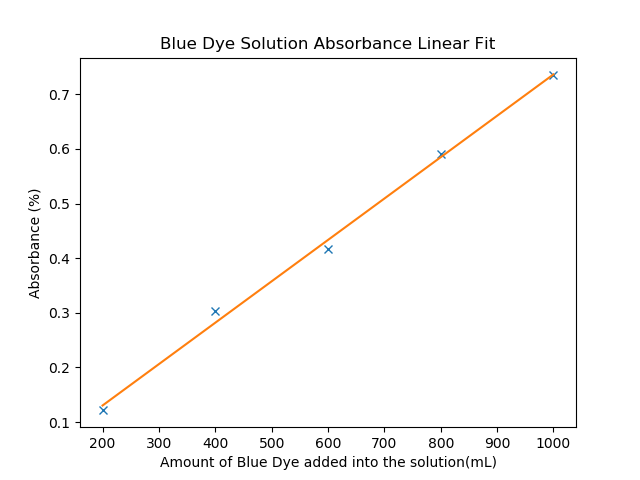
\includegraphics[width = 4 in]{Blue_Dye_Solution_Absorbance_Linear_Fit.png}
    \caption{Blue Solution Absorbance Linear Fit Result}
    \label{fig:my_label}
\end{figure}

The scipy program calculated that the slope of the line is $0.1514$, the interception is $0.13043$, the p value is $8.7006 \times 10^{-5}$, the standard deviation of the data points from the fitted line is $0.0051$.

\begin{figure}[h!]
    \centering
    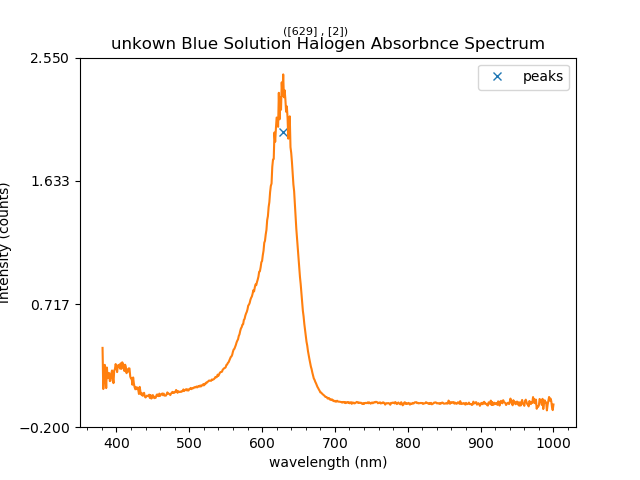
\includegraphics[width = 4 in]{unkown Blue Solution Halogen Absorbnce Spectrum.png}
    \caption{Unkown Blue Solution Halogen Absorbnce Spectrum}
    \label{fig:unkown}
\end{figure}
%% I_0 = 3.749; 
From Python's data analysis program, we can find that the peak absorption happened of the unknown solution happens at wavelength $629 nm$ with an absorption intensity of $2.425$ counts. From Equation 13), our reference data and dark spectrum, we can calculate the absorbance of the blue dye with unknown concentration.

\begin{equation}
    A_{unknown} = 0.452
\end{equation}

With equation 10) from the theory section, we can calculate the concentration based on the linear fit result calculated above.

\begin{equation}
    c_{unknown} = 2.9865 
\end{equation}

%% TODO - figure out the unit of c!!


\subsection{Emission Spectra of Light Sources Results}

\subsubsection{Halogen Lamp and Mercury Vapor Lamp}
The measured emission spectrum of the Halogen lamp is shown in figure~\ref{fig:halogen emission spectrum}.


\begin{figure}[h!]
    \centering
    \includegraphics[width = 4.5 in ]{Halogen_Emission_Spectrum.png}
    \caption{Halogen Lamp Emission Spectrum}
    \label{fig:halogen emission spectrum}
\end{figure}

The measured emission spectrum of the room light is shown in figure~\ref{fig:room light emission spectrum}.

\begin{figure}[h!]
    \centering
    \includegraphics[width = 4.5 in ]{Room_light_emission_spectrum.png}
    \caption{Room Light Emission Spectrum}
    \label{fig:room light emission spectrum}
\end{figure}

The sharpest peaks seem to be at $405 \pm 2$ nanometers, $435 \pm 2$ nanometers, $495 \pm 2$ nanometers, $545 \pm 2$ nanometers, and $610 \pm 2$ nanometers.

\subsubsection{Laser Spectra}
The measured emission spectrum of the red laser is shown in figure~\ref{fig:red laser emission} .

\begin{figure}[h!]
    \centering
    \includegraphics[width = 4.5 in ]{red_laser_emission_spectrum.png}
    \caption{Red Laser Emission Spectrum}
    \label{fig:red laser emission}
\end{figure}

The peak is at 635 nanometers. The FWHM is found to be $2 \pm 1$ nanometers. 

The measured emission spectrum of the green laser is shown in figure~\ref{fig: green laser emission} .

\begin{figure}[h!]
    \centering
    \includegraphics[width = 4.5 in ]{green_laser_emission_spectrum.png}
    \caption{Green Laser Emission Spectrum}
    \label{fig: green laser emission}
\end{figure}

The peak is at 532 nanometers. The FWHM is found to be $2 \pm 1$ nanometers. 

\subsubsection{LED Spectra}
The measured emission spectrum of the red LED is shown in figure~\ref{fig:red LED emission}.

\begin{figure}[h!]
    \centering
    \includegraphics[width = 4.5 in ]{Red_LED_emission_spectrum.png}
    \caption{Red LED Emission Spectrum}
    \label{fig:red LED emission}
\end{figure}

The peak of the red light LED is 690 nm with a FWHM of 70 nm.
The measured emission spectrum of the blue LED is shown in figure~\ref{fig:blue LED emission} .

\begin{figure}[h!]
    \centering
    \includegraphics[width = 4.5 in ]{Blue_LED_emission_Spectrum.png}
    \caption{Blue LED Emission Spectrum}
    \label{fig:blue LED emission}
\end{figure}

The peak of the blue LED is 436 nanometers with a FWHM of 30 nanometers.

The emission spectrum of the yellow LED is shown in figure~\ref{fig:yellow LED emission}.

\begin{figure}[h!]
    \centering
    \includegraphics[width = 4.5 in ]{Yellow_LED_emission_spectrum.png}
    \caption{Yellow LED Emission Spectrum}
    \label{fig:yellow LED emission}
\end{figure}

The emission spectrum of the white LED is shown in figure~\ref{fig:white LED emission}.

\begin{figure}[h!]
    \centering
    \includegraphics[width = 4.5 in ]{White_LED_Emission_Spectrum.png}
    \caption{White LED Emission Spectrum}
    \label{fig:white LED emission}
\end{figure}

\subsubsection{LED Smartphone Flashlights}
The emission spectrum of the iPhone 6+ smartphone flashlight is shown in figure~\ref{fig:iphone LED emission}

\begin{figure}[h!]
    \centering
    \includegraphics[width = 4.5 in ]{Smartphone_Flashlight_Emission_Spectrum.png}
    \caption{iPhone 6+ LED Flashlight Emission Spectrum}
    \label{fig:iphone LED emission}
\end{figure}

The emission spectrum of the Samsung S8 Rugby LED flashlight is shown in figure~\ref{fig:samsung LED emission}

\begin{figure}[h!]
    \centering
    \includegraphics[width = 4.5 in ]{flashlight_emission_sepctrum_samsumg.png}
    \caption{Samsung LED Flashlight Emission Spectrum}
    \label{fig:samsung LED emission}
\end{figure}


\section{Discussion}
\subsection{CCD Integration Time Investigation Discussion}
The effect of changing the CCD Integration Time was found to be analogous to the effects of altering the shutter position of the light source, which limits the amount of photons incident on the CCD. When the light source has a perfectly stable brightness, or the light source is giving off the same amount of photons in each unit of time, the integration time should be directly proportional to the counts registered in the program up until the effect of pixel saturation can be observed. The conclusion of the investigation is that altering the integration time is a tool most useful for avoiding pixel saturation for a given wavelength, which would otherwise obscure the peak wavelength(s) of a spectrum.

\subsection{Absorption and Transmission of Colored Glass Filters Discussion}
The spectra that were recorded showed a lot of noise at lower wavelengths. The noise in the absorbance and transmission spectra 
\subsection{Absorption in Color Additive Solutions Discussion}

\subsection{Emission Spectra of Light Sources Discussion}

\subsubsection{Characterization of Peaks}
The sharpest peaks with the smallest linewidths were the lasers. Lasers should have both Lorentzian and Gaussian elements to their linewidths stemming from the ever-present Heisenberg uncertainty principle as well as thermal effects on the electrons inside the lasing medium causing Gaussian broadening.

The fluorescent mercury vapor room lights also had very narrow linewidths for the peaks 435 and 610 nanometers. These should be Lorentzian in nature, coming from the collisional broadening as well as natural broadening of the pressurized mercury vapor inside the lights.

The LEDs had peaks with much wider linewidths, 



\subsubsection{Spectral Contamination by Room Light}
The spectra of the red laser, the blue, yellow, red and white LEDs, and the desktop monitor displaying white all showed the peaks associated with the room lights. This was due to the measurement taking process. The room lights were left on and were able to reflect off surfaces into the optical cable. 

In the future, in order to measure the spectra of emission sources, more care needs to be taken to exclude the light of all other light sources, beginning with turning off the room lights while other light sources are being measured.
\section{Conclusion}
\section{References}

\bibitem{units}
 "Resolutions of the 26th CGPM". BIPM. November 16, 2018. 
 
\bibitem{labHandout}
  https://www.asp.uni-jena.de/aspmedia/Optics+Training+Laboratory/
  
  Setup+Descriptions/SetupFundamentals.pdf
  \emph{Laboratory Handout}.
  Abbe School of Photonics,
  January 2019
  
\bibitem{Gaussian and Lorentzian and Voigt Picture}
https://scipython.com/book/chapter-8-scipy/examples/the-voigt-profile/

\bibitem{Fluorescent Mercury Vapor Lamp Spectral Peaks}
http://www.euhou.net/index.php/exercises-mainmenu-13/classroom-experiments-and-activities-mainmenu-186/179-observations-of-various-spectra-with-a-home-made-spectroscope

\bibitem{spectra}
Gilbert, Pupa and Haeberli, Willy. \emph{Experiments on subtractive color mixing with a spectrophotometer}. AMER J PHYS. April 2007.
\end{document}
